\documentclass[11pt]{article}
\usepackage[brazil]{babel}
\usepackage[utf8]{inputenc}
\usepackage[T1]{fontenc}
\usepackage{setspace}
\usepackage{epsfig}
\usepackage[pdftex]{hyperref}
\usepackage{multirow,multicol}
\usepackage{fancyhdr,url} 
\usepackage{float}
\usepackage{authblk}%affil , para colocar a universidade
\usepackage[table]{xcolor}
\usepackage[normalem]{ulem} %para "riscar" o texto
\usepackage{amsmath}
\usepackage{indentfirst}
\usepackage{unicode-math}
\usepackage{amssymb}
\usepackage[noabbrev]{cleveref}
\usepackage{caption}


\newcommand{\mudatexto}[1]{\textcolor{red}{#1}}
\newcommand{\duvida}[1]{\textcolor{blue}{#1}}
\newcommand{\obs}[1]{\textcolor{cyan}{#1}}
\newcommand{\afazer}[1]{\textcolor{violet}{#1}}
\newcommand{\atualizado}[1]{\textcolor{teal}{#1}}


%%%%%%%%%%%%%%count enumarete start in zero
\usepackage{enumitem}
\setlist[enumerate,1]{start=1} % only outer nesting level

%%apalike reference
%\usepackage{natbib}
\usepackage[alf,abnt-emphasize=bf]{abntex2cite}


\topmargin -2.0cm 
\headsep 1.5cm   
\oddsidemargin 0.4cm 
\evensidemargin 0.4cm
\textheight = 235mm \textwidth 165mm


\pagestyle{plain}
\usepackage{multicol}
\addtolength\columnsep{2pt}

\newcommand\tab[1][0.5cm]{\hspace*{#1}}


\begin{document}

\pagestyle{fancy}
\lhead{
  
\includegraphics[scale=0.75]{figuras/logo_dcc.pdf}
}
\chead{
  \scriptsize{
    UNIVERSIDADE DO ESTADO DE SANTA CATARINA -- UDESC\\
    CENTRO DE CIÊNCIAS TECNOLÓGICAS -- CCT\\
    DEPARTAMENTO DE CIÊNCIA DA COMPUTAÇÃO -- DCC
  }
}
\rhead{
  \includegraphics[scale=0.75]{figuras/logo_udescjlle.pdf}
}

\title{
Plano de Trabalho de Conclusão de Curso \\
Otimização na seleção de portfólios de investimento utilizando meta-heurística evolutiva e rede neural artificial
}

\author{
UDESC -- Centro de Ciências Tecnológicas\\
Departamento de Ciência da Computação\\
Bacharelado em Ciência da Computação\\
Turma 2020/1 -- Joinville/SC\\
~\\

Paula Campigotto - \texttt{paula\_campigotto@hotmail.com}\\
Omir Correia Alves Junior -\texttt{ omir.alves@udesc.br} {\it (orientador)}\\

}

\date{16 de março de 2020}

\maketitle


\onehalfspacing  %espaçamento de 1,5

%------------------------------------------------
%------------------------------------------------
%------------------------------------------------
%------------------------------------------------
%------------------------------------------------
\begin{abstract}

    A seleção de um portfólio de investimento pode ser classificada como um problema combinatorial multiobjetivo, posto que pretende reduzir o risco de perda e potencializar o retorno esperado. Por demandar um custo computacional impraticável no uso de métodos matemáticos exatos, as principais técnicas utilizadas para a solução deste problema são as meta-heurísticas, as quais fornecem um resultado aproximativo. No entanto, existem outras maneiras de selecionar um portfólio ou refinar tal seleção, como o uso de redes neurais artificiais, uma modelagem que não é tão explorada na otimização de portfólios como as meta-heurísticas. Desta forma, este trabalho pretende comparar a rentabilidade das soluções geradas por um método meta-heurístico e por um modelo que faz uso de redes neurais artificiais. 
    
    \vskip 0.5cm

    \noindent\textbf{Palavras-chave:} \textit{Portfólios de investimento, Otimização multiobjetivo, Redes neurais artificiais, Meta-heurísticas.}

\end{abstract}






%------------------------------------------------
\section{Introdução e Justificativa}
\label{sec:int}

%Seleção de portfolios  %Modern portfolio theory - markowitz

A seleção de um portfólio, ou carteira, de investimentos consiste na combinação de diversos ativos, tais como ações, moedas, \textit{commodities}, títulos públicos ou debêntures, que podem variar de acordo com o perfil do investidor. As principais máximas utilizadas na seleção em otimização de portfólio são a minimização do risco de perda e a maximização do retorno esperado, isto é, espera-se que todo investidor tenha esses dois objetivos a serem alcançados ao realizar um investimento no mercado financeiro. 



Partindo desses pressupostos, \citeonline{Markowitz1952} formulou a Teoria Moderna de Portfólios, que contextualiza o seu problema de otimização, também conhecido como modelo de variância média, o qual objetiva estimar a proporção de ativos que comporão uma carteira de investimentos. Tal modelo recebeu este nome, variância média, por utilizar a variância do portfólio como métrica para o cálculo do risco pelo qual este portfólio está exposto. Harry Markowitz formulou matematicamente seu problema utilizando uma função multiobjetivo, conforme as Equações \ref{eq:1} e \ref{eq:3}, sujeitas às restrições apresentadas nas Equações \ref{eq:2} e \ref{eq:4}.

\begin{equation} \label{eq:1}
\text{min}\sum_{i=1}^{N} \sum_{j=1}^{N} w_{i}w_{j}\sigma_{ij} 
\end{equation}

\begin{equation} \label{eq:3}
    \text{max}\sum_{i=1}^{N} w_{i}\mu_{i} = R
\end{equation}

\begin{equation} \label{eq:2}
\sum_{i=1}^{N} w_{i} = 1
\end{equation}

\begin{equation} \label{eq:4}
    0 \leq w_{i}, w_{j} \leq 1, \qquad i,j = 1, ..., N
\end{equation}

    Na Equação \ref{eq:1} é apresentada a função objetivo que visa a minimização do risco e que é dada pelo somatório da covariância $\sigma_{ij}$ de todos os pares $i$ e $j$ de ativos da carteira, composta por $N$ ativos, multiplicada pelas proporções desses ativos. A covariância $\sigma_{ij}$ é exposta na Equação \ref{eq:5}, em que o valor de $T$ corresponde ao número total de cotações utilizadas. Cada uma dessas cotações pode ser identificada por seu tempo $t$, sendo $t \in \{1, 2, ..., T\}$. O valor de $r_{i}^{t}$ é a taxa de retorno do ativo $i$ no tempo $t$ e pode ser visualizada na Equação \ref{eq:6}. Por fim, $\mu_{i}$ equivale ao retorno esperado do ativo $i$. 

    \begin{equation} \label{eq:5}
        \sigma_{ij} = \frac{1}{T} \sum_{t=1}^{T} (r_{i}^{t} - \mu_{i}) (r_{j}^{t} - \mu_{j})
    \end{equation}
    
    \begin{equation} \label{eq:6}
        r_{t} = \frac{p_{t} - p_{t-1}}{p_{t-1}} \qquad p_{t} = \text{preço do ativo no tempo $t$}
    \end{equation}

    A segunda função objetivo do problema diz respeito à maximização do retorno $R$, apresentado na Equação \ref{eq:3}, e corresponde ao somatório do produto entre a proporção, ou peso, $w_i$ e o retorno esperado $\mu_i$ de cada ativo $i$.
    As restrições impostas pelo problema garantem que o somatório de todas as proporções dos ativos integrantes da carteira sejam igual a 1 (Equação \ref{eq:2}) e que as proporções de cada um dos ativos estejam compreendidas no intervalo $[0,1]$ (Equação \ref{eq:4}).

    %% CVaR
    
    Há outras maneiras para mensurar o risco em portfólios de investimentos, como por exemplo a utilização das métricas \textit{Value at Risk -- VaR} \cite{var} e \textit{Conditional Value at Risk -- CVaR} \cite{Rockafellar2000}, os quais são métodos estatísticos e realizam a ordenação dos retornos do portfólio a fim de encontrar o valor do risco utilizando um nível de confiança $\beta \in (0,1)$ e o número $n$ correspondente ao tamanho da série histórica dos ativos. O \textit{VaR} corresponde ao valor da perda na posição $(1-\beta)n$ da série ordenada, todavia, \citeonline{Rockafellar2002} propuseram o \textit{CVaR}, o qual considera perdas maiores do que o índice do VaR, solucionando este problema que estava presente no cálculo do risco com \textit{VaR}. 
    
    %VaR
    
    \citeonline{Rockafellar2000} definiram a fórmula do \textit{VaR} conforme a Equação \ref{eq:var}, em que $x$ é o portfólio em questão, $\beta$ representa o nível de confiança e $\alpha_{\beta}(x)$ é o menor valor para $\alpha$ quando $\Psi(x,\alpha) = \beta$. A função $\Psi(x, \alpha)$ pode ser visualizada na Equação \ref{eq:psi}, onde $x$ representa o vetor de pesos de ativos em um portfólio, e $y$ é um vetor de incertezas, isto é, a série de perdas ou parâmetros de mercado que podem influenciar a perda, e $p(y)$ é a distribuição de probabilidade de $y$ em $\mathbb{R}$. 
    
    Tendo em vista que o retorno de um portfólio é calculado a partir da soma do retorno de todos os ativos multiplicados por suas respectivas proporções, é possível afirmar que a função de perda $f(x,y)$, apresentada na Equação \ref{eq:loss}, é o oposto do retorno do portfólio. \cite{Rockafellar2000}
    

    
    \begin{equation} \label{eq:var}
        VaR = \alpha_{\beta}(x) = min\{\alpha \in \mathbb{R}: \Psi (x,\alpha) \geq \beta \}
    \end{equation}
    
    \begin{equation} \label{eq:psi}
        \Psi(x,\alpha) = \int\limits_{f(x,y) \leq \alpha}^{} p(y)dy
    \end{equation}
    
    \begin{equation} \label{eq:loss}
        f(x,y) = - [x_{1}y_{1} + ... + x_{n}y_{n}] = x^{T}y
    \end{equation}
    
    Assim, o \textit{VaR} de um determinado ativo em um portfólio é o número correspondente ao valor $(1-\beta)n$ dos retornos após serem ordenados e enumerados crescentemente. Dessa forma, é possível afirmar que o \textit{VaR} corresponde à potencial máxima perda a um intervalo de confiança específico em um tempo determinado e pode ser traduzido como a quantia em que as perdas não se excederão em $(1- \beta)$\% dos cenários. \cite{puc}
    
    O \textit{CVaR} é a métrica de risco representada pela média das perdas considerando o intervalo entre o pior resultado e o \textit{VaR}, possibilitando o conhecimento de informações sobre a extensão das perdas. A Equação \ref{eq:cvar_cont} apresenta o \textit{CVaR} para distribuição contínua, em que $x$ é o portfólio de ativos, $\alpha$ é o percentil da distribuição de $x$ e $f(x)$ é uma função de perda associada à $x$. \cite{Araujo2015}
    
    \citeonline{Rockafellar2000} propuseram uma modificação na Equação \ref{eq:cvar_cont}, a qual é apresentada na Equação \ref{eq:cvar_2}. As variáveis apresentadas são as mesmas mencionadas nas Equações \ref{eq:var}, \ref{eq:psi} e \ref{eq:loss}, referentes ao \textit{VaR}.
    
    \begin{equation} \label{eq:cvar_cont}
        CVaR_{\alpha}(X) = -\alpha^{-1} \int\limits^{VaR}_{\infty} x f(x) dx
    \end{equation}
    
    \begin{equation} \label{eq:cvar_2}
        \phi_{\beta}(x) = (1 - \beta)^{-1} \int\limits_{f(x,y) \geq \alpha_{\beta}(x)} f(x,y) p(y) dy
    \end{equation}


        
    A Equação \ref{eq:cvar_comb} é uma combinação das Equações \ref{eq:var} e \ref{eq:cvar_2}, em termos de uma função $F_{\beta}$, para distribuições contínuas de probabilidade. Para distribuições discretas, há algumas modificações na fórmula, conforme \cite{Araujo2015}, apresentadas na Equação \ref{cvar3}.
        
    \begin{equation} \label{eq:cvar_comb}
        F_{\beta}(x,\alpha) = \alpha + (1-\beta)^{-1} \int\limits_{y \in \mathbb{R}^{m}} [f(x,y) - \alpha]^+ p(y) dy 
    \end{equation}
    
    \begin{equation} \label{cvar3}
        F'_{\beta}(x,\alpha) = \alpha + \frac{1}{n(1-\beta)} \sum_{k=1}^{n}[f(x,y) - \alpha]^+  
    \end{equation}
    
    Dessa forma \citeonline{Araujo2015} definem o modelo de otimização de portfólios utilizando o \textit{CVaR} como medida de risco, conforme a Equação \ref{eq:cvar_modelo} e sujeito às restrições apresentadas nas Equações \ref{eq:2} e \ref{eq:4}. 
    Por definição, em um específico nível de confiança $\beta$, o \textit{VaR} de um portfólio é a menor quantia, $\alpha$, tal que, com uma probabilidade $\beta \in \{0.90, 0.95, 0.99\}$, a perda não excederá $\alpha$. O \textit{CVaR} é a expectativa condicional de perdas acima desse valor $\alpha$. Tais definições garantem que o \textit{VaR} nunca é maior do que o $\textit{CVaR}$, portanto portfólios com baixo \textit{CVaR} devem ter baixo valor de \textit{VaR}. \cite{Rockafellar2000}
    
    \begin{equation} \label{eq:cvar_modelo}
        Min: \alpha + \frac{1}{n(1-\beta)} \sum^{n}_{i=1} [-w_{i}\mu_{i}-\alpha]^+ 
    \end{equation}
    
    %%%%%%%%% revisar alpha e beta (trocados)
    
    A Figura \ref{fig:var_cvar} ilustra a disposição dos retornos de uma carteira de ativos de acordo com a distribuição normal, dessa forma os menores retornos estão mais à esquerda, enquanto que os maiores estão mais à direita. 
    
    \begin{figure}[H]
        \centering
        \caption{VaR, CVaR e perda esperada}
        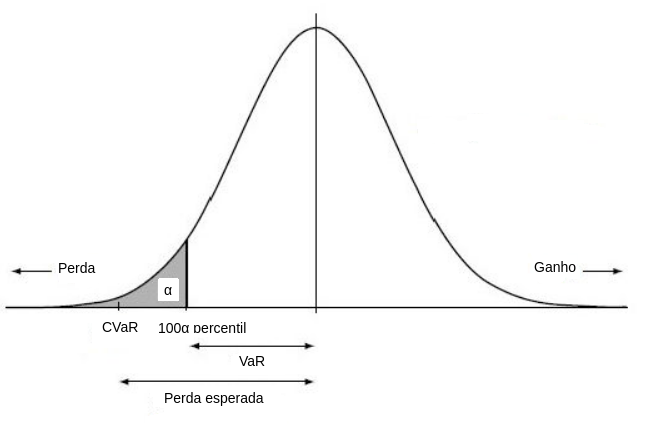
\includegraphics[scale=.53]{figuras/var_cvar.png}
        \caption*{Fonte: \citeonline{yoshiba2002}}
        \label{fig:var_cvar}
    \end{figure}
    
    
    
    
    %Otimização multiobjetivo - NP
    
    O conflito entre as funções objetivo apresentadas pelas Equações \ref{eq:1} e \ref{eq:3}, posto que o retorno de um investimento é proporcional ao seu risco, aumenta a complexidade do problema, impossibilitando a solução a partir de métodos matemáticos exatos, os quais fornecem o melhor resultado possível. É por este motivo que o problema é chamado multiobjetivo, pois caso tais objetivos não fossem conflitantes seria possível o estabelecimento de uma única função, caracterizando um problema mono-objetivo. Tendo em vista que a composição de um portfólio é dada por $n$ ativos com um peso, ou proporção, $w \in [0, 1]$ cada, e sendo $n$ a cardinalidade da carteira, é intuitiva a noção de que tal otimização trata-se de um problema combinatorial, isto é, a diversificação e a complexidade do problema são proporcionais. Assim, a otimização de portfólios com restrição de cardinalidade está contida na classe computacional de problemas $\mathcal{NP}$-difícil\footnote{Os problemas da classe $\mathcal{NP}$ são aqueles que podem ser solucionados, em tempo polinomial, por uma máquina de Turing não determinística e verificados em tempo polinomial por uma máquina de Turing determinística. \cite{danielsson2001}}. \cite{danielsson2001}
    
    %heuristicas - pareto
    
    O processo de otimização consiste em encontrar a melhor solução para um dado problema, utilizando para isto algoritmos eficientes. Os algoritmos podem ser implementados utilizando-se métodos exatos ou não exatos. As técnicas mais utilizadas quando métodos exatos são impraticáveis, como na otimização de portfólios com restrição de cardinalidade, são as heurísticas e meta-heurísticas, as quais produzem resultados que, apesar de aproximados, têm qualidade aceitável \cite{goldbarg}. As heurísticas são técnicas baseadas em experiência para solucionar problemas, fornecendo uma resposta satisfatória em um tempo computacional razoável. As meta-heurísticas estão em um nível superior às heurísticas, posto que elas guiam o \textit{design} das heurísticas a fim de encontrar, gerar ou selecionar uma heurística (algoritmo de pesquisa parcial) que pode fornecer uma solução suficientemente boa para o problema. Assim os algoritmos meta-heurísticos, ao pesquisar sobre um espaço de busca contendo um conjunto de soluções viáveis, podem encontrar boas soluções com menor esforço computacional, comparado aos métodos baseados em cálculo ou heurísticas simples. \cite{metaheuristic}
    
    % heuristicas evolucionarias
    
    Para solucionar certos problemas, a Inteligência Artificial -- IA, na qual estão contidas as heurísticas e meta-heurísticas, utiliza e se inspira em diversas técnicas e conceitos observados na natureza, como exemplo os algoritmos \textit{Simulated Annealing, Ant Colony, Genetic Algorithm}, redes neurais artificiais, dentre outros. Os quais são abstrações das noções de termodinâmica, organização de formigas, biologia evolutiva e sistema nervoso central, respectivamente. A computação explora estes e os demais comportamentos naturais utilizados para resolver problemas e adapta-os para a solução de problemas computacionais e tal ramo da Ciência da Computação é chamado de Computação Natural. \cite{goedert} 
    
    A computação evolucionária se baseia no paradigma neo-Darwinista para simular a evolução natural de sistemas biológicos. Tal paradigma é uma combinação da clássica teoria evolucionária de Darwin, da seleção de Weismann e da genética de Mendel. Um algoritmo evolucionário consiste em um gerador e selecionador de população, um estimador de \textit{fitness} e três operadores genéticos básicos chamados de \textit{cruzamento, mutação} e \textit{seleção}. Dessa forma indivíduos de uma população competem e trocam informações uns com os outros a partir da geração randômica de uma população inicial que sofrerá iterações de cruzamento e mutações para a geração de novas populações até que um pré-determinado critério seja satisfeito de acordo com o estimador de \textit{fitness}. \cite{metaheuristic}
    
    %nsga-II
    
    O algoritmo genético é um algoritmo evolutivo e uma de suas ramificações mais utilizadas em portfólios de investimentos é o \textit{Nondominated Sorting Genetic Algorithm II} -- NSGA II, proposto por \citeonline{nsga2}, o qual é uma evolução de sua primeira versão -- NSGA -- proposta por \citeonline{nsga}. A contribuição do NSGA II sobre o NSGA está em sua complexidade, a qual foi reduzida de $O(N^3m)$ para $O(N^2m)$, em que $N$ é o número de indivíduos e $m$ é o número de funções objetivo.
    
    A Figura \ref{fig:nsga2} ilustra o princípio de funcionamento do NSGA II. Após a criação aleatória da primeira população $P_t$, de tamanho $N$, uma nova população, $Q_t$, também de tamanho $N$, é gerada a partir das operações de seleção, recombinação e mutação sobre $P_t$. A união dessas duas populações forma a população $R_t = P_t \cup Q_t$, de tamanho $2N$, a qual será submetida à ordenação de acordo com os critérios de não-dominação\footnote{O conceito de não-dominação está relacionado com a fronteira de pareto e as funções objetivo do problema, assim, uma solução domina outra quando seu retorno para a função \textit{fitness}, ou objetivo, é melhor do que o retorno da outra.}. Tal ordenação segrega os indivíduos da população, isto é, associa as soluções à diferentes classes -- $F_1, F_2, F_3, ..., F_n$ -- de acordo com o seu elitismo (dominância sobre outras soluções). Dessa forma, os indivíduos pertencentes à classe $F_1$ são as melhores soluções, as quais estarão presentes, por completo, na população $P_{t+1}$ e quanto maior o índice da classe, piores são as soluções nela contidas. Portanto, para a formação da população $P_{t+1}$, de tamanho N, são alocados os indivíduos contidos nas primeiras classes enquanto os demais são rejeitados. Por fim, caso $P_{t+1}$ satisfaça o critério de parada, a solução será retornada, caso contrário $P_{t+1}$ atuará como a população inicial da próxima iteração. \cite{nsga2}
    
    \begin{figure}[H]
        \centering
        \caption{Processo do NSGA II}
        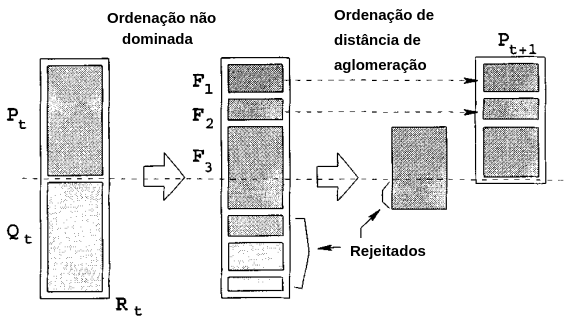
\includegraphics[scale=.6]{figuras/nsga2.png}
        \caption*{Fonte: \citeonline{nsga2}}
        \label{fig:nsga2}
    \end{figure}

    %redes neurais artificiais
    
    Outra técnica contida no segmento da computação natural é a utilização de redes neurais artificiais, que simulam a transmissão de impulsos nervosos entre os neurônios, os quais são representados por nós em um grafo, que por sua vez representa a rede neural. \cite{rn_eng} Os impulsos nervosos são as informações transmitidas entre os nós da rede como entradas e saídas e essa rede pode conter diversas camadas. As camadas de uma rede neural artificial são definidas pela quantidade de nós que a informação de entrada em outro nó já percorreu, isto é, como as saídas dos neurônios podem ser utilizadas como entradas para outros neurônios pode-se estimar a camada em que o nó pertence através do número de nós pelo qual esta informação já foi uma entrada ou saída. \cite{katti} 
    
    
    Os neurônios são as estruturas elementares do sistema nervoso humano e, similarmente, nas redes neurais artificiais, tais estruturas também são chamadas de neurônios, ou nós. Um neurônio artificial consiste em um vetor de múltiplas entradas de valores reais $X = (X_1, ... X_r)^T$ e uma única saída $Y$. Além disso há um vetor $\beta = (\beta_1, ..., \beta_r)$ o qual compreende os pesos de conexão $\beta_i$ entre cada entrada e saída. O valor da saída $Y$ é obtida a partir da Equação \ref{eq:nn_1}, que utiliza o valor de ativação $U$, o qual, por sua vez, é a soma de $X$ com seus respectivos pesos presentes no vetor $\beta$ e está apresentado na Equação \ref{eq:nn_2}. \cite{djehiche}
    
    \begin{equation} \label{eq:nn_1}
        Y = f(U) = f(\beta_0 + X^T\beta)
    \end{equation}
    
    \begin{equation} \label{eq:nn_2}
        U = \beta_0 + \sum^r_{i=1} \beta_iX_i = \beta_0 + X^T \beta
    \end{equation}
    
    Na Equação \ref{eq:nn_1} a função $f(U)$ representa a função de ativação, a qual conecta entradas com a saída de um neurônio. Sua importância está relacionada ao fato de que funções de ativação não lineares são responsáveis por fornecer, às redes neurais artificiais não lineares, a habilidade de modelar funções não lineares e, assim, tais funções podem compactar uma entrada infinita em uma saída finita a partir do mapeamento de $\mathbb{R}$ em um intervalo finito.
    A Figura \ref{fig:neural_network_perceptron} apresenta a arquitetura de um neurônio artificial, conforme a explanação referida.
    
    \begin{figure}[H]
        \centering
        \caption{Modelo de neurônio artificial: perceptron com uma única camada}
        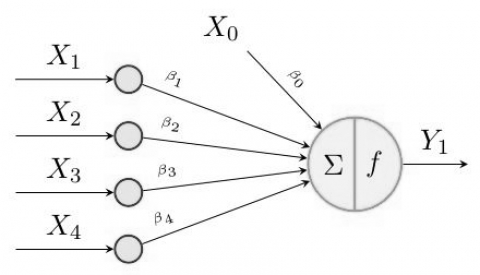
\includegraphics[scale=.6]{figuras/nn.jpg}
        \caption*{Fonte: \citeonline{djehiche}}
        \label{fig:neural_network_perceptron}
    \end{figure}
    
    %trabalhos relacionados
    
    \citeonline{YAMAN2019} propuseram um modelo de rede neural artificial para a solução do problema de otimização em portfólios na bolsa de valores de Istambul. A topologia da rede em questão pode ser visualizada na Figura \ref{fig:nn} e nas Equações \ref{nn1}, \ref{nn2} e \ref{nn3}.
    
    O algoritmo representado pela Figura \ref{fig:nn} realiza operações sobre os vetores $x, y, z, dx, dy$ e $dz$ considerando a média e o desvio padrão das ações. As entradas dos neurônios da rede neural artificial provêm da saída de outros neurônios, caracterizando a retroalimentação da rede. Por fim, se os critérios de parada forem atendidos são calculados o retorno esperado, o risco e a razão de Sharpe\footnote{Uma medida que indica o retorno médio, menos o retorno sem risco, dividido pelo desvio padrão do retorno de um investimento.} do portfólio selecionado com as proporções de $x_i$ utilizando a Equação \ref{nn1}.
    
    \begin{equation} \label{nn1}
        x = -2\sigma(x + kx) + [1,1,...1]^T(y + ky) + \mu^T(z + kz), x > 0 
    \end{equation}
    
    \begin{equation} \label{nn2}
        y = [1,1...1] - [1,1...1](x + kx)
    \end{equation}
    
    \begin{equation} \label{nn3}
        z = -\mu(x + kx) + R, z > 0 
    \end{equation}
    
    \begin{figure}[H]
        \centering
        \caption{Rede neural artificial para otimização de portfólios}
        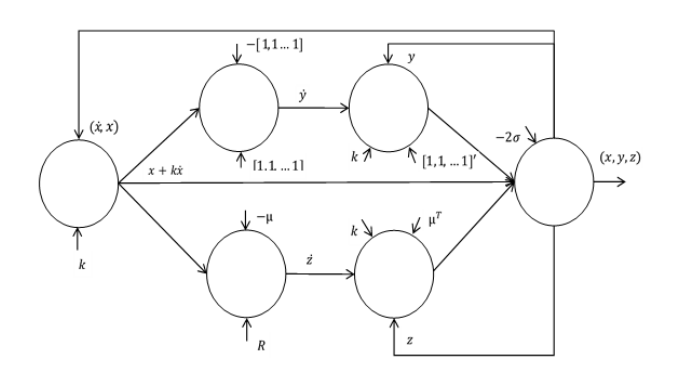
\includegraphics[scale=.5]{figuras/nn_portfolio.png}
        \caption*{Fonte: \citeonline{YAMAN2019}}
        \label{fig:nn}
    \end{figure}
    
    
    \citeonline{cartacho_ufmg} criou um modelo que utiliza redes neurais artificiais para prever os valores futuros de ativos e um algoritmo genético para a otimização do portfólio. Dessa forma, foi realizada uma simulação de investimentos durante os anos de 1999 e 2000, utilizando carteiras compostas por oito ações negociadas na Bovespa durante o ano referido. O processo foi dividido em duas etapas, na primeira foi utilizado o método de Markowitz para a geração do portfólio e na segunda foi utilizado o modelo híbrido criado pelo autor, o qual utilizou redes neurais e um algoritmo genético. \citeonline{cartacho_ufmg} concluiu que os retornos acumulados durante os dois anos de simulação foram de 257,24\% para o método tradicional e 419,41\% para o modelo alternativo. 
    
    \citeonline{nicholas_silva} utilizou, em seu trabalho, os modelos de Harry Markowitz e de Black Litterman para realizar a otimização de portfólios. Ademais, o autor também utilizou a técnica de \textit{clusterização} da área de \textit{machine learning} (algoritmo \textit{KMeans}) e comparou os resultados de portfólios calculados em uma única data e portfólios recalculados a cada dois meses. Foi possível concluir que as carteiras geradas pelo modelo Black Litterman foram os mais beneficiados pelo uso da clusterização, alcançando um bom desempenho em comparação ao índice \textit{S\&P500}.
    
    \citeonline{dametto} teve como objetivo predizer, com maior acurácia, os valores futuros dos ativos presentes na Bovespa, durante oito anos (janeiro de 2010 a dezembro de 2017). Para isso foi comparado e combinado, por meio de ensembles, três técnicas de \textit{machine learning}:
    \begin{enumerate}
        \item Multilayer Perceptrons (MLP)
        \item Modelo Auto-regressivo Não-linear com Entradas Exógenas (NARX)
        \item Long-Short Term Memory (LSTM)
    \end{enumerate}
    O ensemble criado obteve precisão de 70\%, valor inferior às técnicas MLP e NARX, as quais obtiveram 80\% de acurácia, separadamente.
    
   %%%% Objetvo
   
   \begin{figure}
       \centering
       \caption{Diagrama de processos do experimento}
       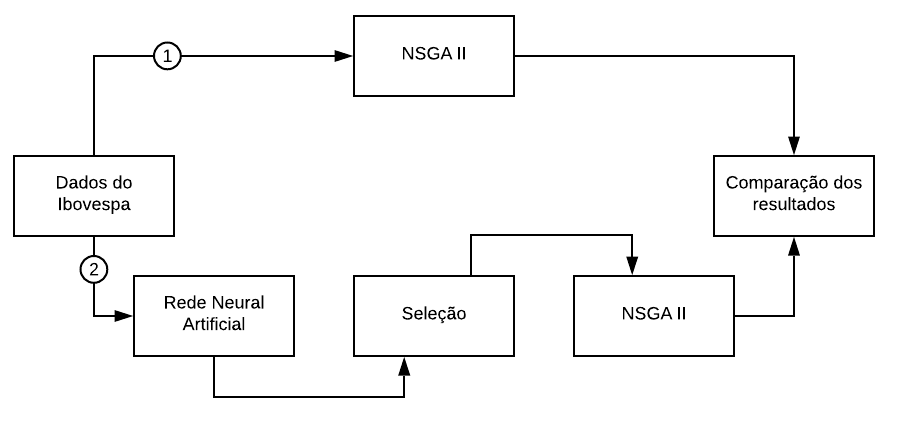
\includegraphics[scale=.5]{figuras/Diagrama_tcc_1.png}
       \caption*{Fonte: Elaborado pela autora (2020)}
       \label{fig:diagrama_processos}
   \end{figure}
   
   A Figura \ref{fig:diagrama_processos} ilustra os processos a serem realizados neste trabalho. Em primeiro lugar serão colhidos os dados históricos dos valores dos ativos cujas ações compõem o Índice da Bolsa de Valores de São Paulo - Ibovespa durante um período de 5 anos (2015 a 2019). Tais dados serão utilizados para a seleção de um portfólio com determinada cardinalidade. Para isso, serão utilizadas duas técnicas diferentes, a primeira delas, indicada pelo número 1 na Figura \ref{fig:diagrama_processos} utilizará o algoritmo NSGA II para selecionar os ativos e suas devidas proporções. A segunda técnica, indicada pelo número 2 na Figura \ref{fig:diagrama_processos}, fará uso de uma rede neural para eleger os melhores ativos, isto é, aqueles que obtiverem o melhor retorno durante a projeção analisada, para que somente depois sejam expostos ao algoritmo NSGA II que indicará quais proporções de cada ativo, gerarão o maior retorno. 
   
   As duas carteiras, montadas pelo algoritmo NSGA II e pela RNA com auxílio do NSGA II, terão seus valores comparados entre si e também entre o Índice Bovespa e outros indicadores financeiros como o CDI - Certificado de Depósito Interbancário, a fim de verificar o desempenho obtido pelas técnicas.
   
   Dado o exposto acima, este trabalho de pesquisa tem como objetivo responder a seguinte pergunta: ``Qual das técnicas apresentadas é capaz de gerar o portfólio de investimentos de melhor qualidade?".
   

%------------------------------------------------
\section{Objetivos}
\label{obj}

    O trabalho visa, de maneira geral, analisar e comparar o desempenho de dois algoritmos na seleção de um portfólio de investimento, tendo como base de dados a série histórica dos valores dos ativos utilizados. Um dos algoritmos será o NSGA-II, o qual se baseia em heurísticas evolutivas, e o outro será uma modelagem de rede neural, utilizando o conceito de aprendizado de máquina em conjunto com o NSGA-II. Ambos os algoritmos estarão embasados na Teoria Moderna de Portfólios, proposta por \citeonline{Markowitz1952} e farão uso do modelo de risco CVaR, modelado por \citeonline{Rockafellar2002}.
   
\subsection{Objetivos específicos}

\begin{itemize}
	\item Realizar a revisão bibliográfica dos conceitos utilizados na monografia, tais como: otimização multiobjetivo, portfólios de investimentos, métricas de risco, algoritmos evolutivos e redes neurais artificiais;
	\item Especificar e implementar um algoritmo de seleção de portfólios utilizando o NSGA-II;
    \item Especificar e implementar um algoritmo de seleção de portfólios utilizando redes neurais;
    \item Realizar os testes dos algoritmos com os dados dos ativos coletados
    \item Analisar os resultados obtidos, comparando com índices financeiros como CDI e Ibovespa;
    \item Comparar o desempenho dos dois algoritmos propostos, quanto a rentabilidade do portfólio selecionado e ao tempo de execução.
\end{itemize}



\section{Metodologia}
\label{met}

    Este trabalho de pesquisa empírica realizará uma análise quali-quantitativa dos experimentos realizados de forma indutiva.

    A elaboração do trabalho partirá de uma revisão bibliográfica dos principais conceitos abordados na pesquisa, tais como a otimização multiobjetivo, teoria moderna de portfólios, heurísticas e meta-heurísticas evolutivas e redes neurais. Similarmente, será realizada uma revisão de trabalhos relacionados ao tema em questão.
    
    Os dados utilizados na pesquisa serão os valores históricos, diários entre 2015 e 2019, das principais ações contidas na Bolsa de Valores de São Paulo e serão obtidos diretamente no \textit{site} da BM\&F Bovespa. Após o tratamento dos dados serão implementados os algoritmos NSGA-II e um modelo de rede neural, os quais fornecerão o possível melhor portfólio de investimento, isto é, que trará melhor rentabilidade. Os algoritmos utilizarão os valores dos 4 primeiros anos (2015 a 2018).
    
    A análise dos resultados será efetuada a partir da verificação do rendimento gerado pelo portfólio selecionado em cada um dos algoritmos no ano de 2019. Tais resultados serão ilustrados em um gráfico de linhas, possibilitando a comparação entre as duas modelagens e também entre outros índices financeiros como o CDI e o Ibovespa. A pesquisa apresentada no trabalho será exploratória e quantitativa, posto que serão realizadas execuções e testes dos algoritmos propostos visando a exploração dos resultados, quantificados, obtidos para a formulação de conclusões sobre o estudo.


    A Tabela \ref{cronograma} apresenta o cronograma que a elaboração do trabalho seguirá durante o ano de 2020, sendo o primeiro semestre dedicado ao TCC 1 e o segundo ao TCC 2. A produção do trabalho, de modo geral, está dividida em 8 etapas, as quais estão indicadas abaixo:

    \begin{enumerate}
    	\item Elaboração do plano do TCC 
    	\item Revisão bibliográfica
    	\item Modelagem do problema
    	\item Escrita do TCC 1
    	\item Implementação dos algoritmos propostos
    	\item Execução dos algoritmos implementados
    	\item Análise dos resultados obtidos
    	\item Escrita do TCC 2
    \end{enumerate}

%------------------------------------------------
\section{Cronograma proposto}
\label{cronograma}

\begin{table}[H]
\caption{Cronograma de atividades} % mude aqui para seu título da tabela
\begin{center}
\tiny 
\resizebox{\textwidth}{!}{ % abre resizebox, setar tabela da largura da página.
%\tabcolsep=0.6cm
\begin{tabular}{|c|l|l|l|l|l|l|l|l|l|l|l|l|} \hline
\multicolumn{1}{|c|}{\multirow{2}{*}{Etapas}} & \multicolumn{6}{c|}{2020/1} & \multicolumn{6}{c|}{2020/2} \\ \cline{2-13}
\multicolumn{1}{|c|}{} & J & F & M & A & M & J & J & A & S & O & N & D \\ \hline
%\rowcolor[HTML]{EFEFEF}
1 & \cellcolor{black} & \cellcolor{black} & ~ & ~ & ~ & ~ & ~ & ~ & ~ & ~ & ~ & ~  \\ \hline
2 & ~ & \cellcolor{black} & \cellcolor{black} & ~ & ~ & ~ & ~ & ~ & ~ & ~ & ~ & ~  \\ \hline
3 & ~ & ~ & \cellcolor{black} & \cellcolor{black} & ~ & ~ & ~ & ~ & ~ & ~ & ~ & ~  \\ \hline
4 & ~ & ~ & ~ & \cellcolor{black} & \cellcolor{black} & ~ & ~ & ~ & ~ & ~ & ~ & ~  \\ \hline
5 & ~ & ~ & ~ & \cellcolor{black} & \cellcolor{black} & \cellcolor{black} & ~ & ~ & ~ & ~ & ~ & ~  \\ \hline
6 & ~ & ~ & ~ & ~ & ~ & ~ & \cellcolor{black} & \cellcolor{black} & ~ & ~ & ~ & ~  \\ \hline
7 & ~ & ~ & ~ & ~ & ~ & ~ & ~ & ~ & \cellcolor{black} & \cellcolor{black} & ~ & ~  \\ \hline
8 & ~ & ~ & ~ & ~ & ~ & ~ & ~ & ~ & \cellcolor{black} & \cellcolor{black} & \cellcolor{black} & ~  \\ \hline
\end{tabular}
 }% fecha resizebox
\end{center}
\label{cronograma} % para referencia no texto.
\caption*{Fonte: (Elaborado pela autora, 2020)}
\end{table}



%------------------------------------------------
%------------------------------------------------ [ GRUPO ]
\section{Linha e Grupo de Pesquisa}

    Este trabalho de conclusão de curso se enquadra na linha de pesquisas de otimização multiobjetivo, meta-heurísticas e aprendizado de máquina. Pertence ao Grupo de Redes e Aplicações Distribuídas (GRADIS), o qual o orientador faz parte.

%------------------------------------------------ [ ORIENTACAO ]
\section{Forma de Acompanhamento/Orientação}

    O acompanhamento do trabalho se dará a partir de reuniões semanais, na sala do professor orientador, localizada no departamento de Ciência da Computação da UDESC, e caso necessário utilizando meios eletrônicos para o esclarecimento de eventuais dúvidas. O controle da orientação é realizado utilizando uma ata de reunião \textit{online} compartilhada entre a aluna e o orientador, a fim de gerenciar a execução do trabalho.



%------------------------------------------------ [ REFERENCIAS ]
% \newpage
%cite on file name apa.bib
% \bibliographystyle{apalike}
\bibliography{sbc-template}
%\nocite{*}
\nocite{cefet, Moreira2018, Castilho2019, Kolm2014, CoelloCoello2006, ashwood, Jaszkiewicz2002, freitas2003, Mansini2015, Araujo2015, Maindonald2009}


\vskip 5cm

\begin{minipage} {0.49\linewidth}
  \centering
  \rule{7.2cm}{0.1mm}

  \textbf{\textit{Omir Correia Alves Junior}}\\
  \textit{(Orientador)}
\end{minipage}
\begin{minipage} {0.49\linewidth}
  \centering
  \rule{7.2cm}{0.1mm}

  \textbf{\textit{Paula Campigotto}}\\
  \textit{(Aluna)}
\end{minipage}

\vskip 1.0cm

\end{document}